\documentclass[11pt,a4paper]{article}
\usepackage[utf8]{inputenc}
\usepackage{amsmath,amssymb,amsthm}
\usepackage{tikz}
\usetikzlibrary{calc}
\usetikzlibrary{math}
\usetikzlibrary{shapes.geometric}
\usetikzlibrary{patterns}
\usetikzlibrary{arrows.meta}
\providecommand{\tikzpicture}{\comment}

\newcommand{\Vnew}{V_{\operatorname{new}}}

\begin{document}

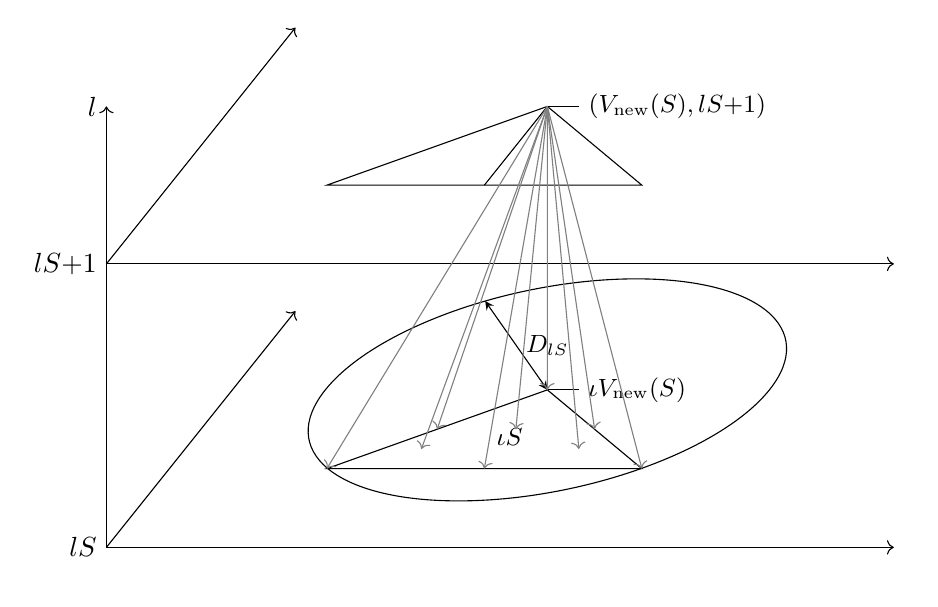
\begin{tikzpicture}[information text/.style={fill=gray!10,inner sep=1ex}, scale=2]
\def\a{1};
\def\b{0};
\def\c{.4};
\def\d{.5};
\def\e{0};
\def\y{1.8};
\def\n{1}
\def\layer{
	\draw[->] (0,0) -- (5,0);
	\draw[->]  (0,0) -- (0,3);
	\draw (1,1) -- (3,1) -- (2,2) -- cycle;
};
\clip (-.5,-.2) rectangle (5.1,3.3);
\draw[->] (0,0) node[left]{$lS$} -- (0,\n*\y+1) node[left]{$l$};

\begin{scope}[cm={\a,\b,\c,\d,(0,\e)}]
	\layer;
	\draw (2,2) -- (2.2,2) node [right]{\small{$\iota\Vnew(S)$}};
	\draw (2,1.4) node {\small{$\iota S$}};
	\coordinate (a) at (1,1){};
	\coordinate (b) at (2,1){};
	\coordinate (c) at (3,1){};
	\coordinate (d) at (1.5,1.25){};
	\coordinate (e) at (2,1.25){};
	\coordinate (f) at (2.5,1.25){};
	\coordinate (g) at (1.5,1.5){};
	\coordinate (h) at (2.5,1.5){};
	\coordinate (i) at (2,1.75){};
	\coordinate (j) at (2,1.5){};
	\coordinate (k) at (2,2){};
	
	\draw (2,2) circle [radius=1.41cm];
	\draw[<->,>=stealth] (2,2) -- node[right] {\small{$D_{lS}$}} (2-1.41*.6,2+1.41*.8);
\end{scope}

\begin{scope}[yshift=\y cm]
\draw (0,0) node[left]{$lS{+}1$};
\begin{scope}[cm={\a,\b,\c,\d,(0,\e)}]
	\fill[white] (0,0) rectangle (5,5);
	\layer;
	\draw (2,2) -- (2.2,2) node [right]{\small{$(\Vnew(S),lS{+}1)$}};
	\draw (2,1)--(2,2);
	\coordinate (A) at (2,2){};
\end{scope}
\end{scope}

\begin{scope}[cm={\a,\b,\c,\d,(0,\e)}]
\foreach\x in {(1,1),(2,1),(3,1),(1.5,1.25),%(2,1.25),
(2.5,1.25),(1.5,1.5),(2.5,1.5),
%(2,1.75),
(2,1.5),(2,2)}
	\draw[->,%>=stealth, 
	gray] (A) -- \x;
\end{scope}


\end{tikzpicture}

\end{document}